\begin{table}
\begin{tabular}{cc}

    \raisebox{-.3\height}{%
        \scalebox{0.7}{%
        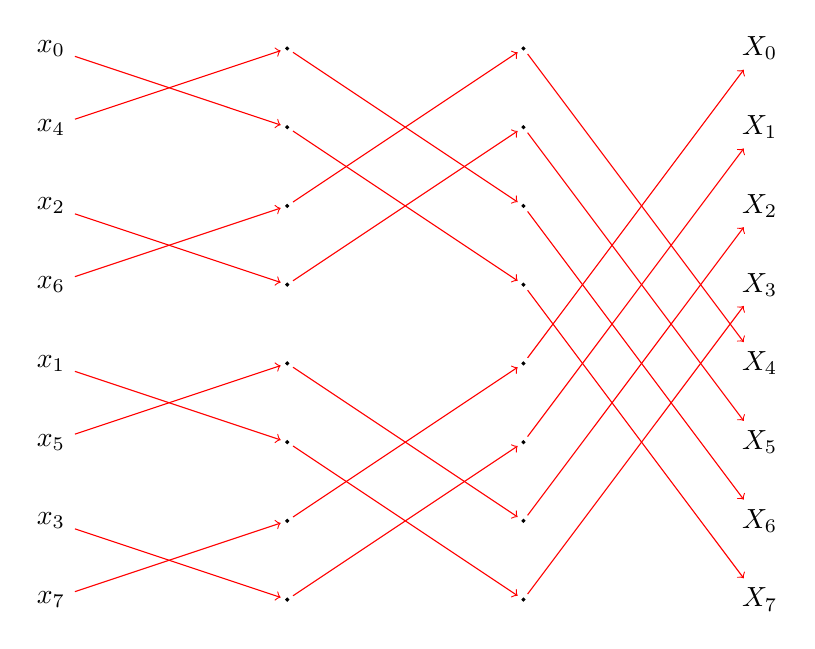
\begin{tikzpicture}[node distance=2cm]
            % nodes
            \node (f0) at (0, 7) {$x_0$};
            \node (f4) at (0, 6) {$x_4$};
            \node (f2) at (0, 5) {$x_2$};
            \node (f6) at (0, 4) {$x_6$};
            \node (f1) at (0, 3) {$x_1$};
            \node (f5) at (0, 2) {$x_5$};
            \node (f3) at (0, 1) {$x_3$};
            \node (f7) at (0, 0) {$x_7$};

            \node [draw,circle,fill=black,inner sep=0pt,outer sep=2pt] (h1) at (3, 7) {};
            \node [draw,circle,fill=black,inner sep=0pt,outer sep=2pt] (h2) at (3, 6) {};
            \node [draw,circle,fill=black,inner sep=0pt,outer sep=2pt] (h3) at (3, 5) {};
            \node [draw,circle,fill=black,inner sep=0pt,outer sep=2pt] (h4) at (3, 4) {};
            \node [draw,circle,fill=black,inner sep=0pt,outer sep=2pt] (h5) at (3, 3) {};
            \node [draw,circle,fill=black,inner sep=0pt,outer sep=2pt] (h6) at (3, 2) {};
            \node [draw,circle,fill=black,inner sep=0pt,outer sep=2pt] (h7) at (3, 1) {};
            \node [draw,circle,fill=black,inner sep=0pt,outer sep=2pt] (h8) at (3, 0) {};

            \node [draw,circle,fill=black,inner sep=0pt,outer sep=2pt] (2h1) at (6, 7) {};
            \node [draw,circle,fill=black,inner sep=0pt,outer sep=2pt] (2h2) at (6, 6) {};
            \node [draw,circle,fill=black,inner sep=0pt,outer sep=2pt] (2h3) at (6, 5) {};
            \node [draw,circle,fill=black,inner sep=0pt,outer sep=2pt] (2h4) at (6, 4) {};
            \node [draw,circle,fill=black,inner sep=0pt,outer sep=2pt] (2h5) at (6, 3) {};
            \node [draw,circle,fill=black,inner sep=0pt,outer sep=2pt] (2h6) at (6, 2) {};
            \node [draw,circle,fill=black,inner sep=0pt,outer sep=2pt] (2h7) at (6, 1) {};
            \node [draw,circle,fill=black,inner sep=0pt,outer sep=2pt] (2h8) at (6, 0) {};

            \node (3h1) at (9, 7) {$X_0$};
            \node (3h2) at (9, 6) {$X_1$};
            \node (3h3) at (9, 5) {$X_2$};
            \node (3h4) at (9, 4) {$X_3$};
            \node (3h5) at (9, 3) {$X_4$};
            \node (3h6) at (9, 2) {$X_5$};
            \node (3h7) at (9, 1) {$X_6$};
            \node (3h8) at (9, 0) {$X_7$};

            % arrows
            % First iteration
            \draw [->,draw=red] (f0) -- (h2);
            \draw [->,draw=red] (f4) -- (h1);
            \draw [->,draw=red] (f2) -- (h4);
            \draw [->,draw=red] (f6) -- (h3);
            \draw [->,draw=red] (f1) -- (h6);
            \draw [->,draw=red] (f5) -- (h5);
            \draw [->,draw=red] (f3) -- (h8);
            \draw [->,draw=red] (f7) -- (h7);

            % Second iteration
            \draw [->,draw=red] (h1) -- (2h3);
            \draw [->,draw=red] (h2) -- (2h4);
            \draw [->,draw=red] (h3) -- (2h1);
            \draw [->,draw=red] (h4) -- (2h2);
            \draw [->,draw=red] (h5) -- (2h7);
            \draw [->,draw=red] (h6) -- (2h8);
            \draw [->,draw=red] (h7) -- (2h5);
            \draw [->,draw=red] (h8) -- (2h6);

            % Third iteration
            \draw [->,draw=red] (2h1) -- (3h5);
            \draw [->,draw=red] (2h2) -- (3h6);
            \draw [->,draw=red] (2h3) -- (3h7);
            \draw [->,draw=red] (2h4) -- (3h8);
            \draw [->,draw=red] (2h5) -- (3h1);
            \draw [->,draw=red] (2h6) -- (3h2);
            \draw [->,draw=red] (2h7) -- (3h3);
            \draw [->,draw=red] (2h8) -- (3h4);
        \end{tikzpicture}
        }%
    }
    &
    \begin{tikzpicture}[node distance=2cm]

        % nodes
        \node (A) at (0, 0) {$x_b$};
        \node (B) at (0, 1) {$x_a$};
        \node (C) at (3, 0) {$x'_b$};
        \node (D) at (3, 1) {$x'_a$};

        \node [draw,circle,above left=-3mm and 2mm of D,inner sep=0pt] (plus) {$+$};
        \node [draw,circle,below left=-3mm and 2mm of C,inner sep=0pt] (plus) {$-$};
        \node [draw,circle,below right=-2mm and 2mm of A,inner sep=0pt] (plus) {$\times$};

        % arrows
        \draw [->,draw=red] (A) -- (D);
        \draw [->,draw=red] (B) -- (C);

    \end{tikzpicture}
\end{tabular}
\caption*{$x'_a = x_a + x_b\omega^{k}_{N}$\\
          $x'_b = x_a - x_b\omega^{k}_{N}$\\\vspace{0.5mm}
         where $\omega^{k}_{N} = e^{-j\frac{2\pi}{N}}$}
\end{table}
